\documentclass[addpoints]{physlabs} % Enable the answers option to display answers to questions.

\labtitle{The Franck-Hertz Experiment}
\labnum{15}
\labnumroman{XV}
\course{PHYSICS 123 - 183}
\coursesubtitle{Waves and Modern Physics}
\date{\today}

\usetikzlibrary{patterns, angles, quotes, shapes, shapes.geometric, arrows.meta, decorations.pathmorphing, hobby}

\begin{document}

\maketitle

% PRELAB SECTION
\begin{prelab}

    \filbreak
    \question[\half] Why should the mercury pressure in the vacuum tube in the Franck-Hertz experiment be low?
    \begin{solution}[3cm]
        We want the electron beam to have the fewest amount of scatters possible from Hg atoms in the tube. If there is too much gas, the beam will not make it to the anode.     
    \end{solution}

    \filbreak
    \question[\half] Draw an atomic model of a ground-state argon atom.
    \begin{solution}[6cm]
        The electron configuration of Ar is $1s^22s^22p^63s^23p^6$, for a total of 18 electrons in three energy levels. Here is a ``solar system'' picture of its structure:
        %
        \begin{center}
            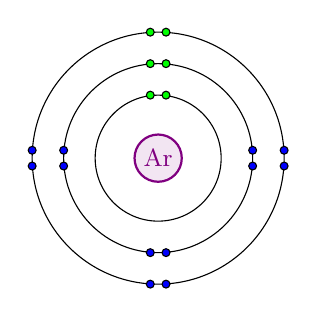
\begin{tikzpicture}
                \draw[thick, violet, fill=violet!10] (0,0) circle[radius=3mm] node {\small Ar};
                % n=1 shell
                \draw (0,0) circle (0.8cm);
                \draw[fill=green] (-0.1,0.8) circle (0.5mm);
                \draw[fill=green] (0.1,0.8) circle (0.5mm);
                % n=2 shell
                \draw (0,0) circle (1.2cm);
                \draw[fill=green] (-0.1,1.2) circle (0.5mm);
                \draw[fill=green] (0.1,1.2) circle (0.5mm);
                \draw[fill=blue, rotate around={90:(0,0)}] (-0.1,1.2) circle (0.5mm);
                \draw[fill=blue, rotate around={90:(0,0)}] (0.1,1.2) circle (0.5mm);
                \draw[fill=blue, rotate around={180:(0,0)}] (-0.1,1.2) circle (0.5mm);
                \draw[fill=blue, rotate around={180:(0,0)}] (0.1,1.2) circle (0.5mm);
                \draw[fill=blue, rotate around={270:(0,0)}] (-0.1,1.2) circle (0.5mm);
                \draw[fill=blue, rotate around={270:(0,0)}] (0.1,1.2) circle (0.5mm);
                % n=3 shell
                \draw (0,0) circle (1.6cm);
                \draw[fill=green] (-0.1,1.6) circle (0.5mm);
                \draw[fill=green] (0.1,1.6) circle (0.5mm);
                \draw[fill=blue, rotate around={90:(0,0)}] (-0.1,1.6) circle (0.5mm);
                \draw[fill=blue, rotate around={90:(0,0)}] (0.1,1.6) circle (0.5mm);
                \draw[fill=blue, rotate around={180:(0,0)}] (-0.1,1.6) circle (0.5mm);
                \draw[fill=blue, rotate around={180:(0,0)}] (0.1,1.6) circle (0.5mm);
                \draw[fill=blue, rotate around={270:(0,0)}] (-0.1,1.6) circle (0.5mm);
                \draw[fill=blue, rotate around={270:(0,0)}] (0.1,1.6) circle (0.5mm);
            \end{tikzpicture}
        \end{center}
    \end{solution}

    \filbreak
    \question[1] Calculate the binding energy of the outermost electron in the Ar atom. According to Bohr's model, the energy of an electron in the $n^\text{th}$ orbital of an atom of atomic number $Z$ is 
    \[
        E = -13.6\frac{Z^2}{n^2}~\text{eV}.
    \]
    \begin{solution}[3cm]
        Argon has $Z=18$ and 3 shells, so according to the Bohr model, ionizing one of the valence electrons requires
        \begin{align*}
            E &= (-\qty{13.6}{eV})\left(\frac{18}{3}\right)^2
               = (-\qty{13.6}{eV})\cdot 36
            \\
              &= \qty{489.6}{eV}.
        \end{align*}
    \end{solution}
    
\end{prelab}

% LAB SECTION
\begin{labsection}

\begin{objective}
    In this lab, you will find the energy required to excite an argon atom from its ground state to its first excited state. This will repeat the experiment of James Franck and Gustav Hertz on mercury, which in 1914 definitively demonstrated the quantum nature of atoms.
\end{objective}

\begin{theory}
    The Franck-Hertz experiment, performed by James Franck and Gustav Hertz in 1914, is the first direct demonstration of the existence of discrete electron energy levels in an atom.
    
    \begin{figure}[ht]
        \centering
        \scalebox{0.9}{\begin{circuitikz}
    % Vacuum tube
    \draw[very thick] (0,0) arc (90:270:2cm);
    \draw[very thick] (0,-4) -- (8,-4);
    \draw[very thick] (8,-4) arc (-90:90:2cm);
    \draw[very thick] (0,0) -- (8,0);
    % Accelerating grid
    \draw[very thick, purple, dash pattern=on 8pt off 3pt] (7,-4) -- (7,0);
    \draw (6,1) node[above,align=left] {accelerating\\grid} -- (6.9,-0.5);
    % Collector (ammeter)
    \draw (9,1) node[above right, align=left] {collector\\(anode)} -- (8.1,-0.75);
    \draw[very thick, blue] (8,-3.5) -- (8,-0.5);
    \draw (8,-2)        
                 to [short] (11,-2)
                 to [rmeter, t=A] ++(0,-3.5)
                 to [battery2, invert, l^={rejecting potential }] ++(-4,0)
                 to [battery2, l^={adjustable voltage (0-\qty{15}{\volt})}, name=Vacc] ++(-8,0)
                 to [battery2, invert, l^={filament supply}] ++(-2,0)
                 to [short] ++(0,5)
                 to [short] ++(2,0)
                 to [L, color=blue] ++(0,-3)
                 to [short, -*] ++(0,-2)
                 ;
    \ctikztunablearrow{1}{1}{220}{Vacc};
    \draw (7,-5.5) to [short, *-] ++(0,1.5);
    % Electrons from electrode
    \draw[blue, thick, densely dotted, -latex] (-0.5,-1.75) -- (2,-1.25);
    \draw[blue, fill=blue] (-0.5,-1.75) circle (0.5mm) node[above] {\small $e^-$};
    \draw[blue, thick, densely dotted, -latex] (-0.25,-2) -- (2.25,-2);
    \draw[blue, fill=blue] (-0.25,-2) circle (0.5mm);
    \draw[blue, thick, densely dotted, -latex] (-0.5,-2.25) -- (2,-2.5);
    \draw[blue, fill=blue] (-0.5,-2.25) circle (0.5mm) node[below] {\small $e^-$};
    % Hg gas inside
    \draw (3,0.5) node[above] {mercury vapor} -- (3.5,-1);
    \draw[violet, fill=violet!10] (5,-3) circle [radius=3mm] node {\small Hg};
    \draw[violet, fill=violet!10] (4,-1) circle [radius=3mm] node {\small Hg};
    \draw[violet, fill=violet!10] (5.5,-2) circle [radius=3mm] node {\small Hg};
    \draw[violet, fill=violet!10] (3,-1.5) circle [radius=3mm] node {\small Hg};
    \draw[violet, fill=violet!10] (3.7,-2) circle [radius=3mm] node {\small Hg};
    \draw[violet, fill=violet!10] (3.4,-3.25) circle [radius=3mm] node {\small Hg};
    % Label the cathode
    \draw (0,1) node [above, align=left] {electron filament\\(at cathode)} -- (-0.75,-1.25);
\end{circuitikz}}
        \caption{A schematic diagram of the original Franck-Hertz vacuum tube.}
        \label{fig: franck-hertz tube}
    \end{figure}
    
    \begin{wrapfigure}[20]{l}{0.35\linewidth}
        
\includegraphics[width=0.95\linewidth]{Lab 15: The Franck-Hertz Experiment/fh-current-vs-voltage.png}
        \caption{Anode current in the vacuum tube ($y$-axis) versus cathode-grid voltage ($x$-axis). Credit: J. Franck and G. Hertz, Verh. Dtsch. Phys. Ges. 16:457, 1914.}
        \label{fig: franck-hertz data}
    \end{wrapfigure}
    
    Franck and Hertz studied energetic electrons traveling through a glass vacuum tube (Fig.~\ref{fig: franck-hertz tube}) filled with a small amount of gaseous mercury (Hg). The electrons were emitted from a hot electrode inside the tube next to a low-voltage contact called the {\bf cathode}. A metal grid held at an adjustable voltage relative to the cathode caused the electrons to accelerate toward the grid. On the far side of the grid, another electrode called the {\bf anode} collected the electrons, allowing Franck and Hertz to measure the current of the electron beam after it passed through the Hg vapor.
    
    As they increased the adjustable voltage, Franck and Hertz found the anode current increased proportionally with the voltage until \qty{4.9}{\volt}, at which point the anode current dropped close to zero. As they continued increasing the voltage beyond \qty{4.9}{\volt}, the current again increased proportionally with the applied voltage until again dropping close to zero at \qty{9.8}{\volt} (exactly twice \qty{4.9}{\volt}). This pattern repeats in steps of \qty{4.9}{\volt}. You can see the pattern in Fig.~\ref{fig: franck-hertz data}, which shows the anode current versus adjustable grid voltage published by Franck and Hertz in 1914.
    
    In a follow-up experiment, Franck and Hertz noticed a blue-violet glow in the Hg gas in the tube, peaking almost entirely at $\lambda=\qty{254}{\nano\meter}$. This wavelength corresponds to a photon energy of
    \[
        E_\text{photon} = \frac{hc}{\lambda} = \frac{(\qty{4.15e-15}{eV~s})(\qty{2.998e17}{\nano\meter/\second})}{(\qty{254}{\nano\meter})} \approx \qty{4.9}{eV}.
    \]
    
    Note that \qty{4.9}{eV} is the kinetic energy of an electron accelerated from rest by a potential difference (or voltage) of \qty{4.9}{\volt}, the same voltage as the period observed with the Franck-Hertz tube (Fig.~\ref{fig: franck-hertz data}). This is not a coincidence. When the accelerated electrons collide with Hg atoms in the gas, at most energies they elastically scatter off the atoms, changing direction but not losing energy. However, at energies of \qty{4.9}{eV}, the electrons collide {\sl inelastically} with the Hg atoms, losing their energy to atomic electrons, which then re-emit the absorbed energy as \qty{254}{\nano\meter} photons. The process is shown schematically in Fig.~\ref{fig: electron-Hg scattering}.
    
    \begin{figure}[ht]
        \centering
        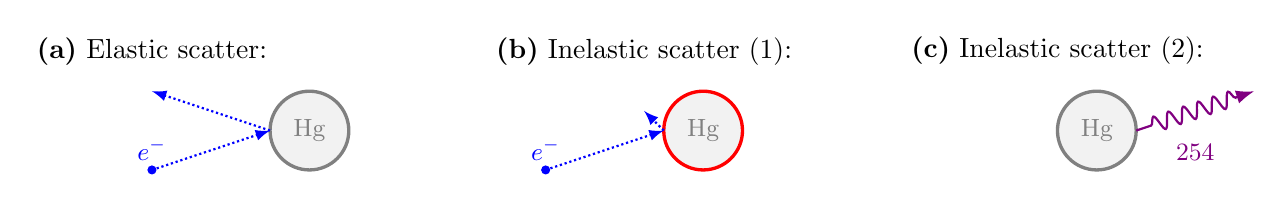
\begin{tikzpicture}[photon/.style={decorate,decoration={snake,post length=2mm,pre length=2mm, segment length=2.0mm, amplitude=1mm,}}]
            % Elastic scatter
            \draw[very thick, gray, fill=gray!10] (0,0) circle [radius=5mm] node {\small Hg};
            \draw[blue, thick, densely dotted, -latex] (-2,-0.5) -- (-0.5,0);
            \draw[blue, thick, densely dotted, -latex] (-0.5,0) -- (-2,0.5) node[above, color=black, yshift=2mm] {{\bf (a)} Elastic scatter:};
            \draw[blue, fill=blue] (-2,-0.5) circle (0.5mm) node[above] {\small $e^-$};
            % Inelastic scatter
            \draw[very thick, red, fill=gray!10] ({0+5},0) circle [radius=5mm] node [color=gray] {\small Hg};
            \draw[blue, thick, densely dotted, -latex] ({-2+5},-0.5) -- ({-0.5+5},0);
            \draw[blue, thick, densely dotted, -latex] ({-0.5+5},0) -- ({-0.75+5},0.25) node[above, color=black, yshift=4.5mm] {{\bf (b)} Inelastic scatter (1):};
            \draw[blue, fill=blue] ({-2+5},-0.5) circle (0.5mm) node[above] {\small $e^-$};
            % UV emission
            \draw[very thick, gray, fill=gray!10] ({0+10},0) node[above, color=black, xshift=-5mm, yshift=7mm] {{\bf (c)} Inelastic scatter (2):} circle [radius=5mm] node [color=gray] {\small Hg};
            \draw [thick, -Latex, violet, photon, use Hobby shortcut] (10.5,0) -- node[midway, below, yshift=-3mm] {\small\qty{254}{\nano\meter}} (12,0.5);
        \end{tikzpicture}
        \caption{In elastic scattering of an accelerated electron from an Hg atom (a), the electron changes direction but loses no energy. In inelastic scattering, the accelerated electron loses \qty{4.9}{eV} to a valence electron in the Hg atom, promoting it from the ground state to the first excited state (b). The valence electron then de-excites and emits a \qty{254}{\nano\meter} photon (c).}
        \label{fig: electron-Hg scattering}
    \end{figure}
    
    In 1913, Niels Bohr published his atomic model of quantized electron energy levels. The Bohr model successfully describes the discrete emission and absorption spectra of hydrogen-like atoms\footnote{Atoms with one electron in the valence shell.}, explaining the spectra as due to transitions of atomic electrons between the quantized energy levels. The Franck-Hertz experiment is consistent\footnote{Note that the Bohr model does not exactly describe the Hg line spectrum, since mercury is not a hydrogenic atom.} with this picture:
    %
    \begin{itemize}
        \item Accelerated electrons in the Franck-Hertz tube collide elastically with Hg atoms at most voltages.
        \item At \qty{4.9}{\volt} and multiples of \qty{4.9}{\volt}, a beam electron inelastically transfers its kinetic energy to a valence electron in atomic mercury, exciting it from the atom's ground state, \ce{Hg(6 ^1S_0)}, to the first excited state, \ce{Hg(6 ^3P_1)}. These two states differ in energy by \qty{4.9}{eV}.
        \item The excited electron then de-excites back to the ground state, causing the emission of a \qty{254}{\nano\meter} photon.
    \end{itemize}
    %
    For his theoretical work on atomic structure, Niels Bohr received the Nobel Prize in Physics in 1922. James Franck and Gustav Hertz were awarded the Nobel Prize in 1925 for their experimental verification of quantized atomic structure.

\end{theory}

\begin{experiment}

    \begin{figure}
        \centering
        \scalebox{0.9}{\begin{circuitikz}
    % Vacuum tube
    \draw[very thick] (0,0) arc (90:270:2cm);
    \draw[very thick] (0,-4) -- (8,-4);
    \draw[very thick] (8,-4) arc (-90:90:2cm);
    \draw[very thick] (0,0) -- (8,0);
    % Accelerating grid G1
    \draw[very thick, purple, dash pattern=on 8pt off 3pt] (1,-4) -- (1,0);
    \draw (0.5,1) node[above,align=left] {accelerating\\grid: G1} -- (0.9,-0.5);
    % Accelerating grid G2
    \draw[very thick, purple, dash pattern=on 8pt off 3pt] (7,-4) -- (7,0);
    \draw (6,1) node[above,align=left] {accelerating\\grid: G2} -- (6.9,-0.5);
    % Collector (ammeter)
    \draw (9,1) node[above right, align=left] {collector\\(anode: A)} -- (8.1,-0.75);
    \draw[very thick, blue] (8,-3.5) -- (8,-0.5);
    \draw (8,-2)        
                 to [short] (11,-2)
                 to [rmeter, t=A] ++(0,-4.5)
                 to [battery2, invert, l^={rejecting potential: $V_\text{G2,A}$}] ++(-4,0)
                 to [battery2, l^={accelerating voltage: $V_\text{G2,K}$ (0-\qty{70}{\volt})}, name=Vacc] ++(-9.5,0)
                 to [short] ++(0,4.5)
                 to [short, -*] ++(0.5,0)
                 ;
    \ctikztunablearrow{1}{1}{220}{Vacc};
    % The electron filament
    \draw (-3.5,-1.25) to[short, o-] ++(2.5,0)
                       to[L, color=blue] ++(0,-1.5)
                       to[short, -o] ++(-2.5,0);
    \draw [latex-latex] (-3.5,-1.35) -- node[midway, fill=white] {$V_\text{H}$} (-3.5, {-1.27 - 1.35});
    % The first accelerating grid
    \draw (-2.5,-5) to[battery2, invert, *-, l_={grid voltage: $V_\text{G1,K}$}] ++(3.5,0)
                    to[short] ++(0,1);
    \draw (7,-6.5) to[short, *-] ++(0,2.5);
    % Electrons from electrode
    \draw[blue, thick, densely dotted, -latex] (-0.5,-1.75) -- (2,-1.25);
    \draw[blue, fill=blue] (-0.5,-1.75) circle (0.5mm) node[above] {\small $e^-$};
    \draw[blue, thick, densely dotted, -latex] (-0.25,-2) -- (2.25,-2);
    \draw[blue, fill=blue] (-0.25,-2) circle (0.5mm);
    \draw[blue, thick, densely dotted, -latex] (-0.5,-2.25) -- (2,-2.5);
    \draw[blue, fill=blue] (-0.5,-2.25) circle (0.5mm) node[below] {\small $e^-$};
    % Hg gas inside
    \draw (3,0.5) node[above] {argon vapor} -- (3.5,-1);
    \draw[cyan, fill=cyan!10] (5,-3) circle [radius=3mm] node {\small Ar};
    \draw[cyan, fill=cyan!10] (4,-1) circle [radius=3mm] node {\small Ar};
    \draw[cyan, fill=cyan!10] (5.5,-2) circle [radius=3mm] node {\small Ar};
    \draw[cyan, fill=cyan!10] (3,-1.5) circle [radius=3mm] node {\small Ar};
    \draw[cyan, fill=cyan!10] (3.7,-2) circle [radius=3mm] node {\small Ar};
    \draw[cyan, fill=cyan!10] (3.4,-3.25) circle [radius=3mm] node {\small Ar};
    % Label the cathode
    \draw (-2.5,1) node [above, align=left] {cathode: K} -- (-2.1,-1.8);
\end{circuitikz}}
        \caption{The tetrode filled with Ar gas used in this lab.}
        \label{fig: franck-hertz argon tube}
    \end{figure}
    
    You will repeat the Franck-Hertz measurement in this lab, but instead of using Hg, we will use a tetrode (a vacuum tube with four penetrating electrodes) filled with argon (Ar) gas. Switching to Ar does not change the nature of the experiment, but it avoids the use of Hg, a neurotoxin that needs to be heated to become a vapor (recall that Hg is a liquid at room temperature).
    
    A schematic view of the setup is shown in Fig.~\ref{fig: franck-hertz argon tube}. In contrast to the original Franck-Hertz device, our setup includes two accelerating grids with separate voltage adjustments. The four electrodes on the device give you control of four settings:\\[-0.5em]
    
    \begin{enumerate}
        \item The potential at the cathode K, which will be connected to ground.
        \item The voltage between the cathode and the first accelerating grid, $V_\text{G1,K}=\qty{1.5}{\volt}$.
        \item The voltage between the cathode and the second accelerating grid, $V_\text{G2,K}=\qty{0}{\volt}$ to \qty{100}{\volt}.
        \item A small rejecting potential $V_\text{G2,A}<\qty{10}{\volt}$ between the second grid and the anode. 
    \end{enumerate}
    %
    By measuring the anode current $I_\text{A}$ with an ammeter, you will characterize the electron beam as a function of the adjustable voltage $V_\text{G2,K}$. You can also change the filament voltage, $V_\text{H}$, to alter the intensity of the electron beam.
    
    \subsection*{Data Collection for the Experiment}
    
    \begin{wrapfigure}{r}{0.4\linewidth}
        \centering
        \setlength{\fboxsep}{0pt}
        \fbox{
\includegraphics[width=\linewidth]{Lab 15: The Franck-Hertz Experiment/fh-scope-trace.png}}
        \caption{Example ocilloscope trace of anode current $I_\text{A}$ versus grid voltage $V_\text{G2,K}$ for Ar.}
        \label{fig: franck-hertz scope trace}
    \end{wrapfigure}
    
    During the experiment, you will start with a low value of $V_\text{G2,K}$. The accelerated electrons in the tube will collide elastically with the Ar gas, so you will see $I_\text{A}$ increasing proportionally with $V_\text{G2,K}$.
    
    When $V_\text{G2,K}$ reaches the first excitation potential\footnote{Experimentally, you'll observe the Ar excitation potential somewhere between \qty{10}{\volt} and \qty{13}{\volt}.} of Ar, the electrons colliding with Ar atoms near grid G2 will interact inelastically with the argon, transferring their kinetic energy to the atoms' valence electrons. The beam electrons will then have too little energy to overcome the reverse field created by the rejecting potential $V_\text{G2,A}$, causing $I_\text{A}$ to drop significantly.
    
    With a further increase of $V_\text{G2,K}$, the beam electrons will be {\bf re-accelerated} by the larger grid voltage after their first inelastic collision with the Ar atoms. The re-accelerated electrons will obtain enough kinetic energy to overcome the reverse field created by $V_\text{G2,A}$, allowing them to reach the anode and causing $I_\text{A}$ to rise proportionally with $V_\text{G2,K}$.
    
    Eventually, $V_\text{G2,K}$ will be twice the excitation potential of Ar, and the electrons re-accelerated to grid G2 will inelastically collide a second time with Ar atoms, losing their energy and causing $I_\text{A}$ to drop again. You can observe this pattern repeating every time $V_\text{G2,K}$ reaches an integer multiple of the excitation potential. An example of how your data will look is shown on the oscilloscope screen capture shown in Fig.~\ref{fig: franck-hertz scope trace}. By measuring the first excitation potential of Ar in this pattern, we verify that the energy absorbed and emitted by the atom is discrete.
    
    \subsection*{Use of the Equipment}
    
    \begin{center}
    \setlength{\fboxsep}{6pt}%
    \setlength{\fboxrule}{2pt}%
    \fbox{\begin{minipage}{0.9\textwidth}
        \color{OrangeRed}
        {\bf WARNINGS}: Read the following directions before using the equipment.
    
        \begin{enumerate}
            \item During the experiment, pay close attention to the output current indicator when the adjustable voltage $V_\text{G2,K}>\qty{60}{\volt}$. This is especially important at the higher voltage (filament voltage) and sensitivity (current multiple) settings. If the current meter reading increases suddenly, decrease the voltage at once to avoid damage to the Franck-Hertz tube.
            %
            \item If you want to change the value of $V_\text{G1,K}$, $V_\text{G2,A}$, and $V_\text{H}$ during the experiment, {\bf first rotate the ``0-100~V'' voltage adjustment knob counter-clockwise all the way to the end} to turn off the grid voltage before making your changes.
            %
            \item The filament voltage of this instrument is $V_\text{H}=\qty{3}{\volt}$, \qty{3.5}{\volt}, \qty{4}{\volt}, \qty{5}{\volt}, \qty{5.5}{\volt}, and \qty{6.3}{\volt}. You can experiment with these filament voltages, but beware that too high a filament voltage can cause current distortion. In such a condition, $V_\text{H}$ should be decreased.
        \end{enumerate}
    \end{minipage}}
    \end{center}
    
    \subsection*{Procedure}
    
    \subsubsection*{Adjust the Operating Voltages}
    
    \begin{enumerate}
        \item Make yourself familiar with the control knobs and read the warning carefully before starting the experiment. Due to the risk of damage to the tube, the use of filament voltage $V_\text{H}>\qty{5}{\volt}$ \textbf{is discouraged} except under the direct supervision of a TA/TI.
    
        \item Make sure the setup has a vacuum tube installed (ask the TA if unsure) and covered prior to use.
        
        \item The 0-100~V knob is continuously adjustable with a soft stop. Use care to \textbf{slowly rotate} this knob during use and when zeroing. Turn all voltage adjustment knobs fully counterclockwise (make all zero). Turn the ``Manual-Auto'' switch to ``Manual'' and rotate the ``Scan Knob'' counterclockwise all the way to the end.
        
        \item \textbf{Set the filament voltage $\mathbf{V_H=4~V}$ and the ``Current Multiple'' selector to $\mathbf{10^{-8}}$}. Turn on the device: the green power indicator will glow. \textbf{Preheat the bulb for 2 minutes before starting your experiment.}\\[-1em]
        
        \textbf{Warning: NEVER change the ``Current Multiple'' selector with the instrument powered on.}\\
        When turning the unit off, the current meter will dip and hold under zero momentarily while the device is powering down.
        
        \item Set $\mathbf{V_{G1,K}=1.5~V}$:\\
        Move the ``Voltage Stepper'' switch to 1.3–5~V, and rotate the 1.3–5~V adjustment knob until the voltmeter reads \qty{1.5}{\volt}.
        
        \item Set $\mathbf{V_{G2,A}=7.5~V}$:\\
        Move the ``Voltage Stepper'' switch to 1.3–15~V, and rotate the 1.3–15~V adjustment knob until the voltmeter reads \qty{7.5}{\volt} (rejecting voltage).
    \end{enumerate}
    
    \subsubsection*{Operation in Manual Mode (OPTIONAL)}
    
    Skip to the next section unless you are explicitly asked by the TA to run in manual mode.
    
    Once you have completed the voltage setup described above, move the ``Voltage Stepper'' switch to 0-100~V and rotate the 0-100~V adjustment knob until the voltmeter reads \qty{0}{\volt} to set $V_\text{G2,K}=\qty{7.5}{\volt}$ (accelerating voltage). Normally, this is fully counterclockwise. Remember that this knob is continuously adjustable with a soft zero. Now you can gradually increase $V_\text{G2,K}$ and record measurements of $I_\text{A}$ with the ammeter and voltmeter.
    
    \subsubsection*{Operation in AUTO Mode (DEFAULT)}
    
    \begin{enumerate}
        \item Complete the voltage adjustment steps described above.
    
        \item Turn on the oscilloscope. Press the \textbf{Menu} button and set it to \textbf{XY} mode by using buttons on the right side of the display.
    
        \item Set up marker channel using the \textbf{Cursor} button. Once you set it properly, the X and Y markers control could be changed using the \textbf{Off} button.
    
        \item Set the trigger on X channel using the \textbf{Trigger} panel on the right side of the scope.
    
        \item Connect the oscilloscope to the Franck-Hertz kit as shown in Fig.~\ref{fig: franck-hertz hookup}. Connect the instrument X output to channel 1 of the oscilloscope and the Y output to channel 2 of the oscilloscope. Don't forget that you also have to connect the instrument's ground to the ground of the oscilloscope.
    
        \begin{figure}[ht]
            \centering
            \setlength{\fboxsep}{0pt}%
            \fbox{
\includegraphics[width=0.8\linewidth]{Lab 15: The Franck-Hertz Experiment/fh-experiment-hookup.png}}
            \caption{Oscilloscope probe connection to the voltage panel of the Franck-Hertz kit.}
            \label{fig: franck-hertz hookup}
        \end{figure}
    
        \item Move the \textbf{Voltage Stepper} on the Franck-Hertz kit to 0–100~V and the operation switch to \textbf{Auto}. If you have connected everything properly signal should look as shown in Fig.~\ref{fig: franck-hertz scope trace}.
    
        \begin{figure}[ht]
        \centering
        \setlength{\fboxsep}{0pt}%
        \fbox{
\includegraphics[width=0.5\linewidth]{Lab 15: The Franck-Hertz Experiment/fh-experiment-scopetrace.png}}
        \caption{Oscilloscope display of an auto-scanned signal from the Franck-Hertz kit.}
        \label{fig: franck-hertz scope trace}
    \end{figure}
    
        \item Measure the peak-to-peak voltage differences using the oscilloscope cursors and fill in Data Table~\ref{data: franck-hertz voltages} in the Postlab exercises.
    
        \item You can also save your data in a flash drive in a different format. For that, use the \textbf{Acquire} button on the top panel.
    
    \end{enumerate}

\end{experiment}

\end{labsection}

% POSTLAB SECTION
\begin{postlab}

    %%% Data Acquisition
    \fullwidth{\subsection*{Data Acquisition - AUTO Mode (\pointsinrange{acquisition} points)}}
    \begingradingrange{acquisition}

    \filbreak
    \question[7] Using the vertical cursor on the oscilloscope, measure the voltage spacing between adjacent dips in the trace.

    \begin{tabular}{lp{3cm}l}
         Location of first dip = & & V \\
         \cline{2-2}
    \end{tabular}

    \begin{center}
        \renewcommand{\arraystretch}{2}
        \captionsetup{font=normalsize}
        \captionof{data table}{Voltage period measurements from the Franck-Hertz Kit. \label{data: franck-hertz voltages}}
        \begin{tabular}{|c|>{\centering\arraybackslash}p{5cm}|>{\centering\arraybackslash}p{4cm}|}
            \hline
            \rowcolor{gray!20}
            Pairs of dips & $\Delta V = V_{i+1} - V_i$ [V] & Average $\Delta V$ [V]
            \\
            \hline
            1-2 & & \\ \cline{1-2}
            2-3 & & \\ \cline{1-2}
            3-4 & & \\ \cline{1-2}
            4-5 & & \\ \cline{1-2}
            5-6 & & \\ \cline{1-2}
            6-7 & & \\ \cline{1-2}
            7-8 & & \\ \hline
        \end{tabular}
    \end{center}

    \filbreak
    \question
    \begin{parts}
        \part[\half] Calculate the standard deviation in average voltage spacing.
        \begin{solution}[3cm]
        
        \end{solution}
        
        \part[\half] What does average voltage spacing physically correspond to?
        \begin{solution}[3cm]
        
        \end{solution}
    \end{parts}

    \filbreak
    \question[2] Sketch the current versus grid voltage as seen in the oscilloscope. Add a title, axis labels, and units.\\[-1em]
    
    Alternatively, you can save the oscilloscope window in picture format and attach it to your hand-in.\\[0em]

    \begin{center}
    \captionsetup{font=normalsize}
    \captionof{graph}{Current versus grid voltage $V_\text{G2,K}$. \label{graph: franck-hertz voltages}}
    % Oscilloscope grid
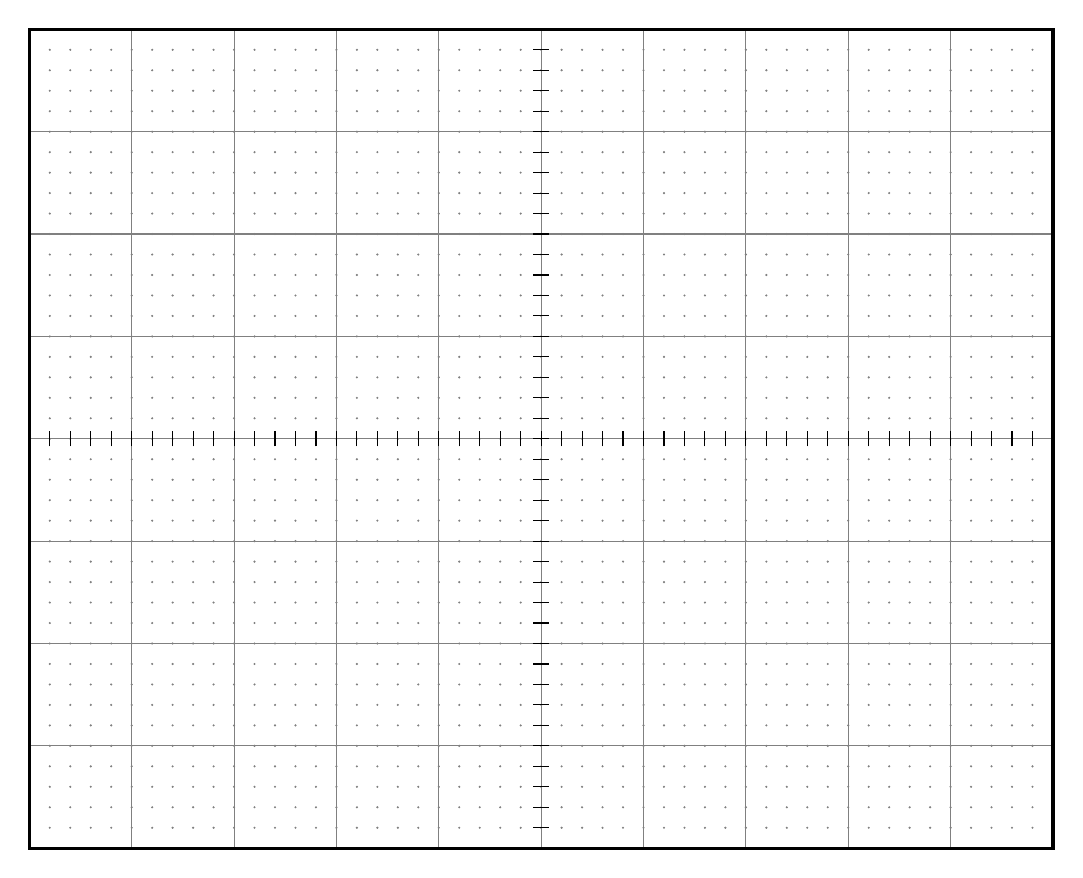
\begin{tikzpicture}
    % Define dimensions
    \def\gridwidth{10}
    \def\gridheight{8}
    \def\spacing{1.3}
    % Draw grid paper on the left
    \begin{scope}[xshift=0cm, yshift=0cm]
        % Grid points
        \foreach \x in {0,2,...,100}
        {
            \foreach \y in {0,2,...,80}
            {
                \draw[gray, fill=gray] (\x*\spacing/10, \y*\spacing/10) circle (0.05mm);
            }
        }
        % Major grid lines
        \foreach \x in {0,1,...,\gridwidth}
            \draw[gray] (\x*\spacing,0) -- (\x*\spacing,\gridheight*\spacing);
        \foreach \y in {0,1,...,\gridheight}
            \draw[gray] (0,\y*\spacing) -- (\gridwidth*\spacing,\y*\spacing);
        \draw[black, very thick] (0,0) rectangle (\gridwidth*\spacing,\gridheight*\spacing);
        % Center gridlines
        \foreach \x in {0,2,...,100}
            \draw (\x*\spacing/10, 3.925*\spacing) -- (\x*\spacing/10, 4.075*\spacing);
        \foreach \y in {0,2,...,80}
            \draw (4.925*\spacing, \y*\spacing/10) -- (5.075*\spacing, \y*\spacing/10);
    \end{scope}
\end{tikzpicture}
    \end{center}

    \endgradingrange{acquisition}

    %%% Data analysis
    \newpage
    \fullwidth{\subsection*{Data Analysis (\pointsinrange{analysis} points)}}
    \begingradingrange{analysis}
    
    \filbreak
    \question[1] How much energy is required to excite an electron in the valence shell of Argon to its first excited state?
    %
    \begin{solution}[4cm]
        
    \end{solution}

    \filbreak
    \question[2] Atoms do not stay in their excited states for long. After some time, the excited Ar atoms return to the ground state by releasing excess energy in the form of electromagnetic radiation. If you were to measure the frequency of radiation from your Franck-Hertz experiment, what would be the frequency?
    %
    \begin{solution}[5cm]
        
    \end{solution}

    \filbreak
    \question[2] Suppose you want to excite Ar to the first excited state by shining electromagnetic radiation on it. What should be the wavelength of the radiation?
    %
    \begin{solution}[3cm]
        
    \end{solution}

    \filbreak
    \question[1] If everything went correctly, you should have seen the higher-order dip current does not reach that of the first few. What could be the reason?
    %
    \begin{solution}[3cm]
        
    \end{solution}

    \filbreak
    \question[1] How might contamination of other gases in the tube affect your result?
    %
    \begin{solution}[3cm]
        
    \end{solution}

    \filbreak
    \question[3] What is your overall conclusion about energy levels in the atom/atomic model from this experiment? Describe its connection to Bohr’s atomic model.
    %
    \begin{solution}[5cm]
        
    \end{solution}

    \endgradingrange{analysis}
    
\end{postlab}

\end{document}